\section{Bibliotecas de aprendizado de máquina}
\label{bibliotecas}
\index{Aprendizado de máquina}
\index{Inteligência artificial}

Considerando apenas a parte matemática por trás de toda esta teoria que fundamenta todo o meio de inteligência artificial e aprendizado de máquina, existe por si só, uma complexidade gigantesca. Implementar modelos e algoritmos populares do zero, tomaria um tempo grande e está sujeito a diversos problemas caso testes específicos não sejam propriamente realizados. 

Dada tamanha dificuldade, bibliotecas e \textit{frameworks} de matemática computacional voltadas para aprendizado de máquina foram desenvolvidos por pesquisadores(as) e engenheiros(as) e disponibilizados ao público geral. Estas ferramentas, abstraem algoritmos e estruturas de uma maneira a eliminar esta complexidade do desenvolvimento de modelos. Isto possibilita que as pessoas foquem seus esforços em desenvolver o modelo mais apropriado e otimizado para o contexto, ao invés de se preocuparem com problemas já resolvidos e bastante testados. 

Diversas bibliotecas estão disponíveis para tais aplicações, muitas delas são de código aberto e têm a visibilidade de uma grande comunidade. Isso permite com que problemas sejam encontrados com antecedência e sugestões de melhoria sejam constantes. As duas ferramentas mais populares durante a escrita deste trabalho para aprendizado de máquina e inteligência artificial são \textit{Pytorch} e \textit{Tensorflow}.

Ambas bibliotecas permitem criar uma rede neural como exemplificado na imagem \ref{fig:exemplo_rede_neural} em uma linguagem de alto nível, como o diagrama \ref{fig:exemplo_rede_neural_diagrama_alto_nivel} mostra.

\begin{figure}[H]
    \centering
    \caption{Exemplo de rede neural.}
    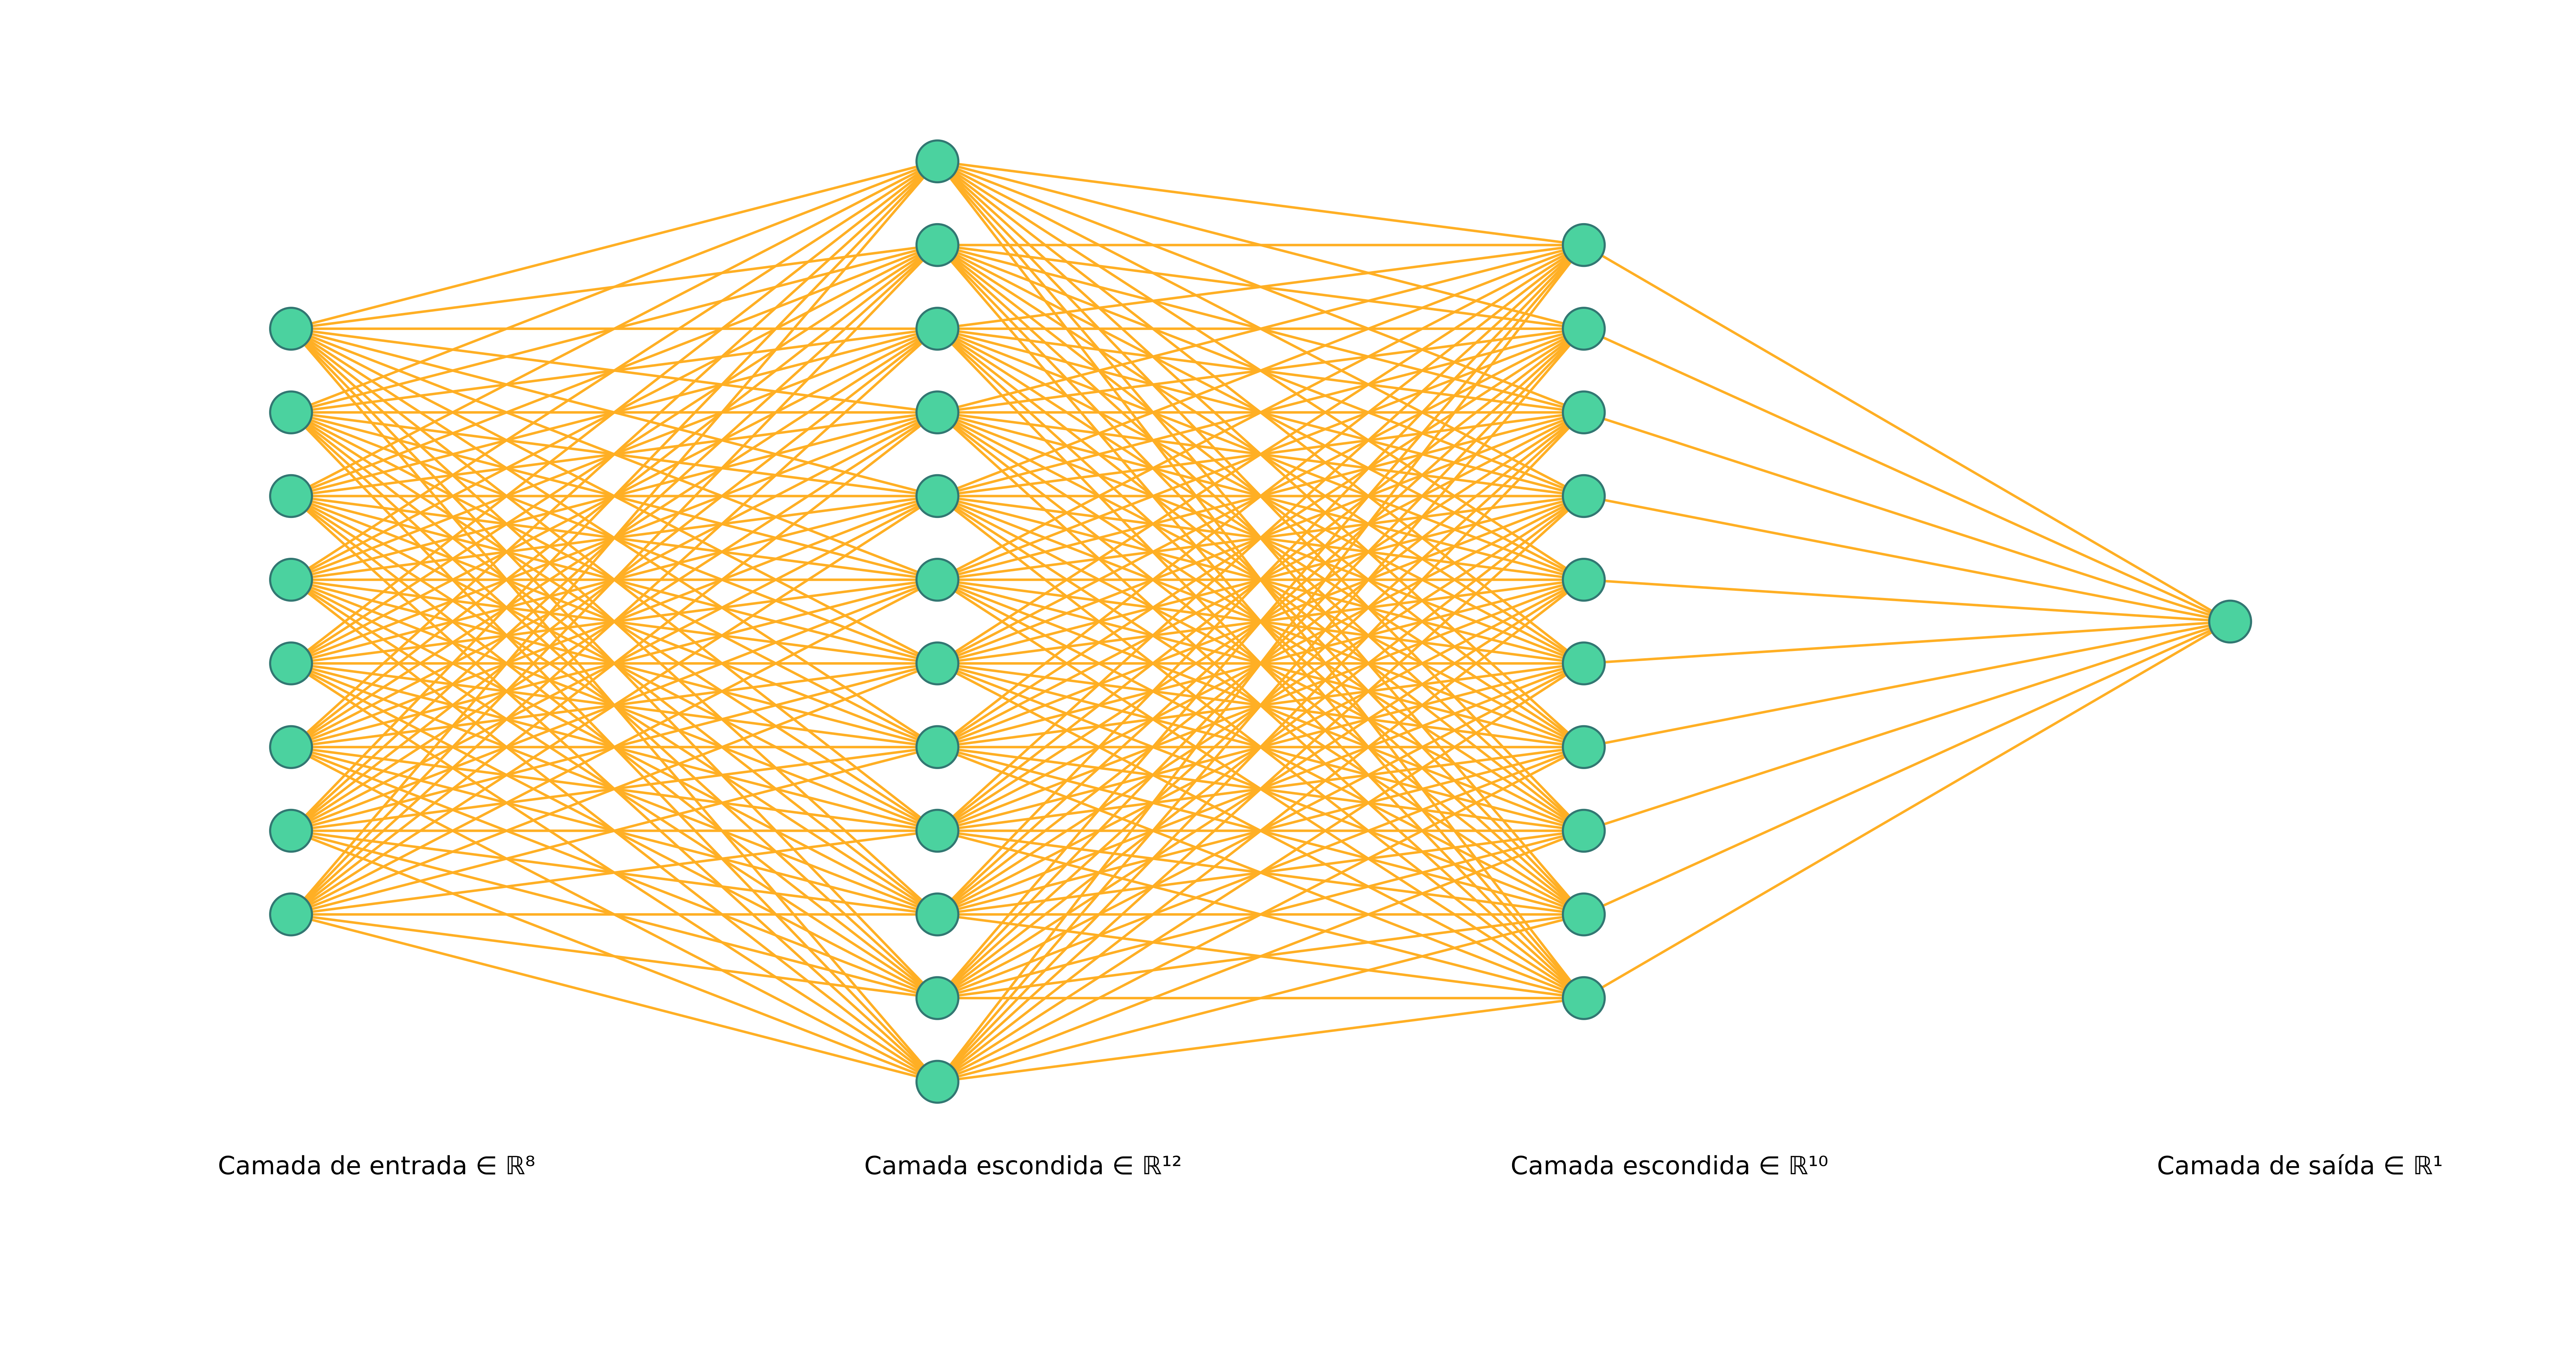
\includegraphics[width=14cm]{fig/nn_8_12_10_1.png}
    \legend{Fonte: Autor, gerada por \cite{lenail_nn_2023}.}
    \label{fig:exemplo_rede_neural}
\end{figure}

\begin{figure}[H]
    \centering
    \caption{Exemplo de rede neural definida em linguagem de alto nível.}
    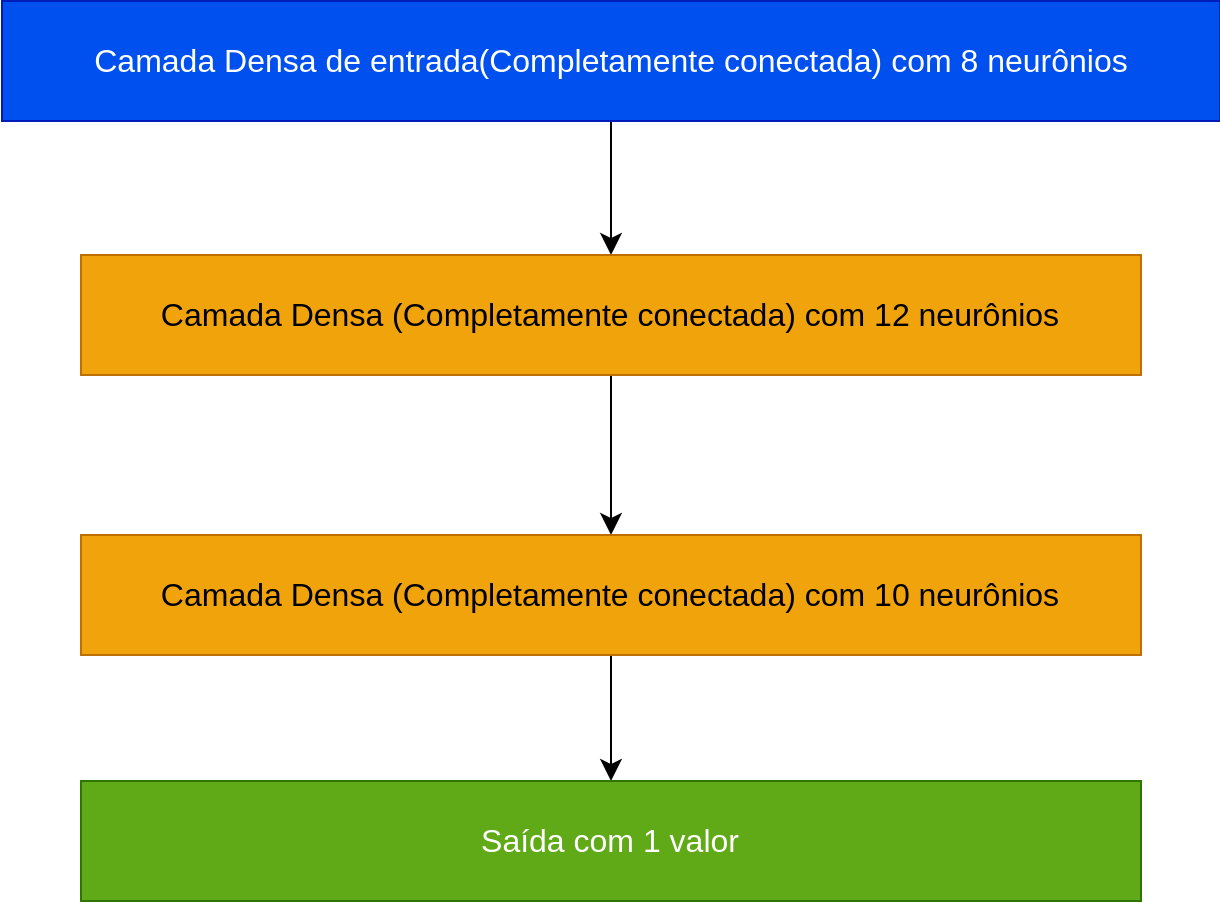
\includegraphics[width=8cm]{fig/sample_nn.png}
    \legend{Fonte: Autor.}
    \label{fig:exemplo_rede_neural_diagrama_alto_nivel}
\end{figure}

Além de dar acesso à uma maneira relativamente simples de desenvolver modelos menos sofisticados, como demonstrado nas figuras \ref{fig:exemplo_rede_neural} e \ref{fig:exemplo_rede_neural_diagrama_alto_nivel}, o \textit{Tensorflow} também fornece acesso à outros níveis de abstração. Desde o mais baixo, onde pessoas que realmente entendem a biblioteca a fundo têm controle total, até o mais alto, onde utilizamos de objetos (como uma camada) previamente desenvolvido e testado, como blocos para construir os modelos finais.

\subsection{Pytorch}
\label{pytorch}
\index{Pytorch}

\textit{Pytorch}, é uma biblioteca de computação de tensores otimizada, baseada na biblioteca \textit{Torch}, capaz de executar em CPUs e em GPUs \cite{pytorch_pytorch_2023}. Foi originalmente desenvolvido pela atual empresa Meta, porém hoje, em código aberto, faz parte da fundação Linux \cite{zemlin_welcoming_nodate}. 

Alguns produtos famosos que fazem uso do \textit{Pytorch} em seu software são o auto-piloto dos carros da \textit{Tesla} \cite{karpathy_pytorch_2019}; \textit{Pyro}, uma linguagem de programação probabilística desenvolvido pela empresa \textit{Uber} \cite{goodman_uber_2017}, entre outros.

\subsection{Tensorflow}
\label{tensorflow}
\index{Tensorflow}

\textit{Tensorflow} é uma biblioteca inicialmente desenvolvida pelo \textit{Google} como parte do projeto \textit{Google Brain}. Foi disponibilizada como código aberto em 2015 \cite{jeff_tensorflow_2015, abadi_tensorflow_2015}. Diversas aplicações utilizam o \textit{Tensorflow}, como o \textit{Google RankBrain} \cite{davies_complete_2020}, um motor de busca baseado em aprendizado de máquina. O \textit{Spotify}, utiliza \textit{Tensorflow} para recomendações e busca de música para seus usuários \cite{ngahane_winding_2019}.
